% One session from start to finish: where each hook runs, and what it shows or stops.
% Colours come from src/styles/palette.json via the generated ../_palette.tex (npm run tokens).
% Shared house style for the TikZ diagrams. render.sh defines \theme (light|dark) before \input.
\documentclass{article}
\usepackage{fontspec}
\usepackage{tikz}
\usepackage{fontawesome5}
\usetikzlibrary{positioning,calc,arrows.meta,fit,backgrounds}
\setmainfont{CrimsonPro}[Path=\fontdir, Extension=.ttf, UprightFont=*, ItalicFont=*-Italic, UprightFeatures={RawFeature={+wght=400}}, ItalicFeatures={RawFeature={+wght=400}}, BoldFont=*, BoldFeatures={RawFeature={+wght=600}}, Scale=1.08]
\setmonofont{JetBrainsMono}[Path=\fontdir, Extension=.ttf, Scale=0.86]
\newfontfamily\kickerfont{JetBrainsMono}[Path=\fontdir, Extension=.ttf, Scale=0.72, LetterSpace=12]
% GENERATED from src/styles/palette.json by scripts/tokens/build.mjs. Do not edit; run `npm run tokens`.
\def\darktheme{dark}
\ifx\theme\darktheme
  \definecolor{ink}{HTML}{EFEFE8}
  \definecolor{muted}{HTML}{A0A09A}
  \definecolor{paper}{HTML}{1B1B19}
  \definecolor{accent}{HTML}{5FE08F}
  \definecolor{accentfill}{HTML}{173322}
  \definecolor{oxide}{HTML}{FF6A4D}
\else
  \definecolor{ink}{HTML}{111111}
  \definecolor{muted}{HTML}{4A4A4A}
  \definecolor{paper}{HTML}{FFFFF8}
  \definecolor{accent}{HTML}{1F7A45}
  \definecolor{accentfill}{HTML}{E6F1EA}
  \definecolor{oxide}{HTML}{C8361C}
\fi

\tikzset{
  every picture/.style={line cap=round, line join=round, font=\normalsize, text=ink},
  card/.style={draw=ink!70!paper, line width=0.6pt, fill=paper, rounded corners=3pt, align=left,
               text width=#1, inner xsep=7pt, inner ysep=5.5pt, anchor=north west},
  card/.default=3.9cm,
  hot/.style={card=#1, draw=accent, line width=1.1pt, fill=accentfill},
  hot/.default=3.9cm,
  ghost/.style={card=#1, draw=muted!80!paper, dashed, fill=none, text=muted},
  ghost/.default=3.9cm,
  panel/.style={draw=muted!45!paper, line width=0.5pt, rounded corners=5pt, inner sep=9pt},
  hotpanel/.style={panel, draw=accent!75!paper, line width=0.9pt},
  line/.style={-{Stealth[length=5pt,width=4.2pt]}, line width=0.7pt, draw=ink!70!paper},
  hotline/.style={line, draw=accent, line width=1pt},
  ghostline/.style={line, draw=muted!80!paper, dashed},
  badline/.style={line, draw=oxide, line width=1pt},
  lbl/.style={font=\small\itshape, text=muted, inner sep=2.5pt},
  head/.style={font=\itshape, text=muted, anchor=south west, inner sep=0pt, align=left},
  warm/.style={card=#1, draw=accent!60!paper, fill=accentfill!50!paper},
  warm/.default=3.9cm,
}
\newcommand{\kicker}[1]{{\kickerfont\MakeUppercase{#1}}}
\newcommand{\ico}[1]{\makebox[1.25em][l]{#1}}
\newcommand{\cardtext}[2]{{\ttfamily #1}\\[1pt]{\small\itshape\color{muted}#2}}
% Crop the page to the picture: typeset it into a box and ship that box as the page.
\newcommand{\diagram}[1]{%
  \setbox0\hbox{#1}%
  \pagewidth=\dimexpr\wd0+8pt\relax \pageheight=\dimexpr\ht0+\dp0+8pt\relax
  \hoffset=-1in \voffset=-1in
  \shipout\vbox{\kern4pt\hbox{\kern4pt\box0}}}

\begin{document}
\diagram{\begin{tikzpicture}[x=1cm,y=1cm]
  \def\U{0.9}\def\H{5.1}\def\G{9.7}\def\R{14.6}\def\E{-11.5}
  \newcommand{\two}[2]{{\upshape\ttfamily\color{ink}#1}\\ #2}
  % phase bands
  \foreach \t/\b/\name in {-0.45/-1.8/start, -1.9/-6.95/during, -7.05/-11.5/finish} {
    \fill[muted!7!paper, rounded corners=4pt] (-0.3,\t) rectangle (16.0,\b);
    \node[font=\kickerfont\scriptsize, text=muted, rotate=90, anchor=south] at (-0.35,{(\t+\b)/2}) {\MakeUppercase{\name}};
  }
  % actors and lifelines
  \foreach \x/\ic/\name/\sty in {\U/user/you/card, \H/shield-alt/hooks/hot, \G/robot/agent/card, \R/code-branch/repo/card} {
    \draw[ink!30!paper, line width=0.6pt, dash pattern=on 2pt off 2pt] (\x,0) -- (\x,\E);
    \node[\sty=1.6cm, anchor=south, align=center] at (\x,0) {\faIcon{\ic}\ \ \name};
  }
  % START
  \draw[hotline] (\H,-1.45) -- node[lbl, above, align=center] {\two{SessionStart}{git log, WORKLOG and the ledger}} (\G,-1.45);
  % DURING
  \draw[line] (\U,-2.45) -- node[lbl, above, pos=0.3] {``compare usage across strains''} (\G,-2.45);
  \draw[hotline] (\H,-3.55) -- node[lbl, above, align=center] {\two{UserPromptSubmit}{the ledger, again}} (\G,-3.55);
  \draw[badline, dashed] (\G,-4.65) -- node[lbl, above, align=center] {\two{Write usage\_plot.py}{in the repo root}} (13.95,-4.65);
  \node[text=oxide] at (14.25,-4.65) {\faIcon{ban}};
  \draw[badline] (\H,-5.75) -- node[lbl, above, align=center] {\two{PreToolUse}{blocked: it goes in experiments/}} (\G,-5.75);
  \draw[line] (\G,-6.6) -- node[lbl, above] {{\upshape\ttfamily\color{ink}Write exp-0015/run.py}} (\R,-6.6);
  % FINISH
  \draw[line] (\G,-7.6) -- node[lbl, above] {``I'm done''} (\H,-7.6);
  \draw[badline] (\H,-8.7) -- node[lbl, above, align=center] {\two{Stop}{not logged, not committed}} (\G,-8.7);
  \draw[line] (\G,-9.55) -- node[lbl, above] {append to WORKLOG, git commit} (\R,-9.55);
  \draw[line] (\G,-10.35) -- node[lbl, above] {``I'm done''} (\H,-10.35);
  \draw[hotline] (\H,-11.15) -- node[lbl, text=accent, above] {\faIcon{check}\ \ allowed} (\U,-11.15);
\end{tikzpicture}}
\end{document}
